\documentclass{article}[18pt]
\usepackage{../../../../../format}
\lhead{MCS - DMLA}


\begin{document}
\begin{center}
\underline{\huge Paths, Cycles, Trees}
\end{center}
\section{Eulerian Circuits}
\subsection{Definition}
A circuit through a graph G so that we start and finish at the same vertex and traverse each edge exactly once

\subsection{Theorem}
A connected graph with at least two vertices has an Eulerian circuit iff each of its vertices has an even degree
\subsection{Idea of Proof}
Necessity ($\Rightarrow$): each time this circuit passes through a vertex v, it contributes 2 to deg(v). Since each edge is used exactly once, deg(v) must be even\\
Sufficiency ($\Leftarrow$): Induction on the number of vertices in G.\\
Induction base: G=$K_3$, the claim is obvious. Induction step:
\begin{itemize}
	\item Start walking from any vertex u along the untraversed edges, marking off the traversed edges
	\item Stop when you arrive at a vertex where you can't continue (all edges leading from it are already traversed). This vertex must be u again
	\item Hence we have a circuit C. Delete all edges in C from G to obtain a smaller graph H where all degrees are also even
	\item By induction hypothesis, each connected component of H has an Eulerian circuit
	\item Combine C and these circuits to obtain the required circuit for G
\end{itemize}
\section{Hamiltonian Cycles}
\subsection{Definition}
A cycle where we start and finish at the same vertex and visit each vertex exactly once
\subsection{Example}
\begin{center}
	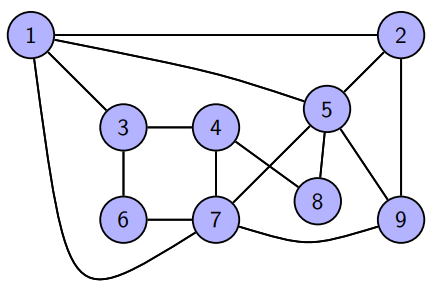
\includegraphics[scale=0.7]{Hamiltonian}
\end{center}
\begin{itemize}
	\item Does this graph has a Eulerian circuit? - No
	\item Does it have a Hamiltonian cycle? - Yes
	\item Detecting Eulerian circuits algorithmically is easy (How?) - compute degrees
	\item Detecting Hamiltonian cycles is hard (NP-Complete)
\end{itemize}

\section{Travelling Salesman Problem}
The TSP is the following problem:
\begin{itemize}
	\item A salesman should visit cities $c_1,c_2,...,c_n$ in some order, visiting each city exactly once are returning to the starting point
	\item A (positive integer) cost d(i,j) of travel between each pair $(c_i,c_j)$ is known
	\item Goal: find an optimal (i.e. cheapest) route for the salesman
\end{itemize}
Given a graph G with a set V of vertices ($|V|=n$) and a set E of edges
\begin{itemize}
	\item for each vertex v, create a city $c_v$
	\item For each pair of distinct $u,v\in V$, set $d(c_u,c_v)=1$ if $uv\in E$ and $d(c_u,c_v)=2$ otherwise
\end{itemize}
Then detecting a hamiltonian cycle in G can be viewed as TSP:
\begin{itemize}
	\item If G has a Hamiltonian cycle then the cycle is a route of cost exactly n
	\item If there is a route of cost n then it can't use pairs with cost 2 and so goes through edges of G and hence is a Hamiltonian cycle
\end{itemize}
\section{Trees}
\subsection{Definitions}
\textbf{Forest} - An acyclic graph, i.e. graph \textbf{without cycles}\\
\textbf{Tree} - A connected forest, i.e. a connected acyclic graph
\subsection{Spanning trees}
$$G ^ { \prime } = \left( V ^ { \prime } , E ^ { \prime } \right) \text { of a graph } G = ( V , E ) \text { is spanning if } V ^ { \prime } = V$$
\subsubsection{Theorem}
Every connected graph contains a spanning tree, i.e., a spanning subgraph that is
a tree.
\subsubsection{Proof}
Let G be a connected graph:
\begin{itemize}
	\item If G contains no cycles, it is a tree, and hence a spanning tree of itself
	\item If G contains a cycle, we can remove one edge from the cycle
	\item The new graph is still connected (Why?)
	\item Repeating this we can destroy all cycles and end up with a spanning tree
\end{itemize}
It follows that trees are the smallest connected structures
\subsection{Leaves}
A left in a tree is a vertex of degree 1
\subsubsection{Lemma}
Every tree on at least 2 vertices contains a leaf
\subsubsection{Proof}
By contraposition:
\begin{itemize}
	\item Assuming that every vertex has degree 0 or at least 2, we will show that the graph is not a tree
	\item If a vertex has degree 0, then the graph (which contains at least 2 vertices) is not connected, hence not a tree
	\item If every vertex has degree at least 2, just start at a vertex, go to one if its neighbours, from there go to another neighbour etc
	\item Since the vertex set is finite, at some stage we encounter a vertex we have already visited
	\item This implies that the graph contains a cycle, so is not a tree 
\end{itemize}
\subsection{Edges of trees}
How many edges does a tree on n vertices have?
\subsubsection{Theorem}
A connected graph on n vertices is a tree iff it has n-1 edges
\subsubsection{Proof}
($\Rightarrow$) Show, by induction on n, that a tree on n vertices has n-1 edges:
\begin{itemize}
	\item For small n the lemma holds: a tree on one vertex has no edges; a tree on two vertices has one edge
	\item Suppose that each tree on n-1 vertices has n-2 edges (induction hypothesis)
	\item Take a tree on n vertices, for some $n\geqslant 3$
	\item T contains a leaf v. Consider the graph T-v, it has one vertex less and one edge less than T
	\item T-v is still connected and (still) acyclic
	\item T-v is a tree with n-1 vertices, by induction hypothesis it has n-2 edges
	\item T has one edge more, so n-1 edges
\end{itemize}
($\Leftarrow$)
\begin{itemize}
	\item Assume that G is a connected graph with n vertices and n-1 edges
	\item Then, as we proved before, G contains a spanning tree T
	\item By the first part of the proof, T contains exactly n-1 edges
	\item T is a subgraph of G, and it has the same number of edges as G
	\item Hence, T and G are the same
	\item In particular, G is a tree
\end{itemize}
\subsection{Paths in trees}
Since a tree is a connected graph, between any two vertices in a tree there is a path, can there be more than one path between two vertices in a tree?
\subsubsection{Lemma}
Let T be a tree and $u,v\in V(T)$ with $u\neq v$\\
Then there is a unique path in T between u and v
\subsubsection{Proof}
By contradiction:
\begin{itemize}
	\item There is a path between u and v in T, since T is connected
	\item Suppose there are two paths P and Q in T between u and v, and derive a contradiction
	\item Let x and y in V(T) be distinct and chosen in such a way that x and y are both P and Q, but between x and y the vertices on P and Q are disjoint. (It is possible that x=u and y=v, but this is not necessarily the case)
	\item Then the segments of P and Q between x and y together form a cycle
	\item This contradicts that T is a tree. Hence there is a unique (u,v) path in T
\end{itemize}
\subsection{Rooted trees}
\subsubsection{Definition}
A rooted tree is a tree in which one vertex is fixed as the root(vertex) (and every edge is directed away from this root)
\subsubsection{Example}
We usually draw a rooted tree in (horizontal) levels, starting with the root (level 0), then the neighbours of the root (level 1), etc
\begin{center}
	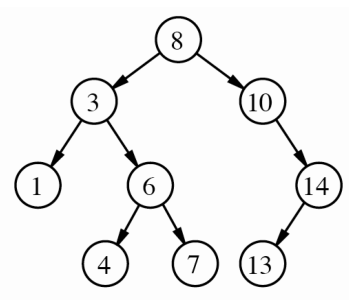
\includegraphics[scale=0.7]{root}
\end{center}
\subsection{Rooted trees, children and parents}
Let v be a vertex in a rooted tree T
\begin{itemize}
	\item The neighbours of v in the next level are called the \textbf{children} of v
	\item The (unique) neighbour of v in the previous level (if v is not the root) is called the \textbf{parent} of v
	\item If v has no children then it is called a \textbf{leaf} of T
	\item If v has children, then it is called an \textbf{internal vertex}
\end{itemize}
\end{document}